\subsection{Método de desarrollo}

El proyecto seguirá una metodología de desarrollo por etapas, en la \acrfull{edt} (figura \ref{fig:edt}) puede verse su estructura.

\begin{figure}[!htp]
	\centering
	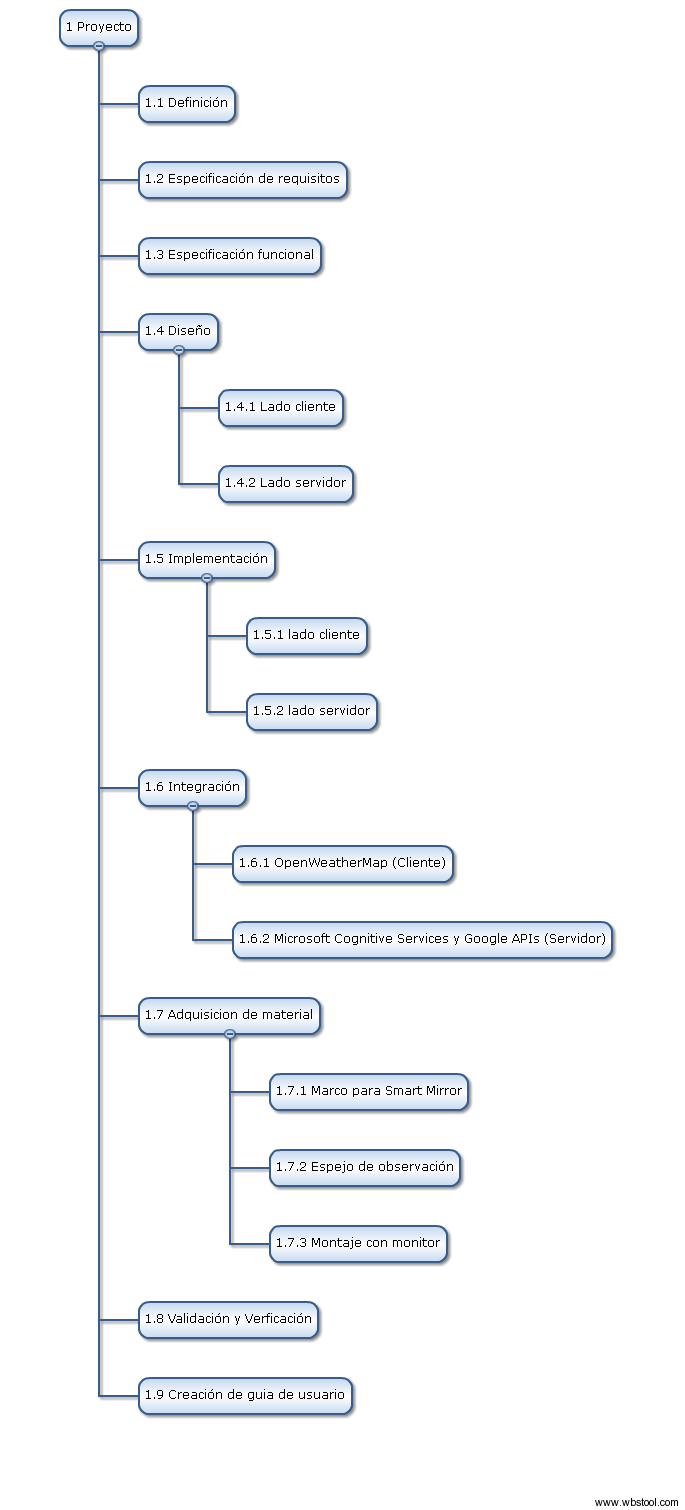
\includegraphics[angle=0, scale=.5]{fig/EDT}
	\caption{EDT}\label{fig:edt}
\end{figure}

Este desarrollo por etapas incluye las siguientes:

\begin{enumerate}
	\item \textbf{Plan operativo:}

	Etapa donde se define el problema a resolver, las metas del proyecto, las metas de calidad y se identifica cualquier restricción aplicable al proyecto.

	\item \textbf{Especificación de requisitos:}

	Permite entregar una visión de alto nivel sobre el proyecto, poniendo énfasis en la posibilidad de una planificación de los recursos sobre una escala de tiempos.

	\item \textbf{Especificación funcional:}

	Especifica la información sobre la cual el software trabajará.

	\item \textbf{Diseño:}

	Permite describir como el sistema va a satisfacer los requisitos.

	\item \textbf{Implementación:}

	Codificación del software.

	\item \textbf{Validación y verificación:}

	Etapa en la que se determina si el software desarrollado cumple con las especificaciones.
	
	\item \textbf{Mantenimiento:}

	Realización de arreglos y mejoras en el software desarrollado.

\end{enumerate}